\documentclass[oneside,numbers,spanish]{ezthesis}

\author{Pablo Maximiliano Lulic}
\title{Proxy Adaptativo Para Protocolos Web Avanzados}
\degree{Licenciatura en Sistemas de Informaci\'on}
\supervisor{Mg. Gabriel Tolosa}
\institution{Universidad Nacional de Luj\'an}

\usepackage{glossaries}
\usepackage{longtable}
\loadglsentries{otros/glosario}
\makeglossary

\hyperlinking
\begin{document}

%titulo	
\begin{titlepage}
  \TitleBlock{\scshape\insertinstitution}
  \TitleBlock{\Huge\scshape\inserttitle}
  \TitleBlock{\scshape
    Trabajo Final presentado por \insertauthor \\
    para obtener el grado de \insertdegree}
     %\TitleBlock{
\includegraphics[height=2cm]{img/logo_unlu}}
  \TitleBlock{\insertsubmitdate}
\end{titlepage}




%prefacio
\prefacesection{Agradecimientos}

...
%mis viejos, euge, gabriel y marce, compa�eros laburo

%Indices y listas de contenido
\tableofcontents
%\listoffigures
%\listoftables		

%Cap'itulos
\chapter{Introducci'on}

El protocolo HTTP tuvo su primera versi'on en mayo de 1996, culminando en 1999 con el est'andar actual que es HTTP 1.1. Es un protocolo sin estado, lo que conlleva a que se necesite realizar una conexi'on nueva por cada recurso que se necesite en un sitio.

Los sitios web de la actualidad difieren de las p'aginas de hace m'as de 10 a'nos, tanto en tama'no como en cantidad de recursos. Este fen'omeno hace que el protocolo ya no tenga el mismo rendimiento que en 'epocas anteriores. A pesar del avance de la tecnolog'ia en cuanto a mejoras en las velocidades de los enlaces de red, un ancho de banda grande no es el 'unico factor que interviene en la performance de la carga de las p'aginas.
Google propuso un protocolo llamado SPDY que busca mejorar la performance de HTTP. Permite m'ultiples streams en una conexi'on simple de TCP, adem'as de otras caracter'isticas como push y hint.
Aprovechando los resultados favorables de las mediciones de este nuevo protocolo, se busca realizar un proxy que maneje SPDY hacia los nodos interiores, y que hacia la world wide web maneje un algoritmo inteligente que pueda determinar seg'un el perfil del sitio que m'etodo (\textsc{http}, \textsc{https} 'o \textsc{spdy}) elegir para mejorar la performance. 

\chapter{Desarrollo de la Web Actual}
\label{desarrolloWeb}
\section{Introducci'on}

Internet es la interconexi'on global de redes individuales alrededor del mundo. Originalmente fu'e utilizada para interconectar laboratorios dedicados a investigaci'on gubernamental. Desde 1994 se expandi'o para millones de usuarios de todo el mundo que la utilizan con m'ultiples prop'ositos. A medida que iba creciendo, cambiaba la forma de hacer negocios y de comunicarse. Hasta llegar a ser una fuente de informaci'on Universal para millones de personas \citep{iws}.

Internet contin'ua creciendo d'ia a d'ia. Hacia 1995 la cantidad de usuarios promedio era de 16 millones, 1 a'no despu'es, la cifra ascendi'o a m'as del doble. Para el a'no 2000 se increment'o 10 veces la cantidad de usuarios. Esta informaci'on puede verse en el Cuadro \ref{cuadroCrecInternet}.

\begin{longtable}{l c c}
\hline
 Fecha & Usuarios(mill) & \% Poblaci'on Mundial\\
\hline \hline
\endfirsthead

\hline
 Fecha & Usuarios(mill) & \% Poblaci'on Mundial\\
\hline \hline
\endhead

\multicolumn{3}{l}{Sigue en la p'agina siguiente.}
\endfoot

\endlastfoot

\hline
Diciembre, 1995 & 16 & 0.4 \\
Diciembre, 1996 & 36 & 0.9 \\
Diciembre, 1997 & 70 & 1.7 \\
Diciembre, 1998 & 147 & 3.6 \\
Diciembre, 1999 & 248 & 4.1 \\
Diciembre, 2000 & 361 & 5.8 \\
Agosto, 2001 & 513 & 8.6 \\
Septiembre, 2002 & 587 & 9.4 \\
Diciembre,  2003 & 719 & 11.1 \\
Diciembre,  2004 & 817 & 12.7 \\
Diciembre,  2005 & 1018 & 15.7 \\
Diciembre, 2006 & 1093 & 16.7 \\
Diciembre, 2007 & 1319 & 20.0 \\
Diciembre, 2008 & 1574 & 23.5 \\
Marzo, 2009 & 1596 & 23.8 \\
Junio, 2009 & 1669 & 24.7 \\
Septiembre, 2009 & 1734 & 25.6 \\
Diciembre, 2009 & 1802 & 26.6 \\
Junio, 2010 & 1966 & 28.7 \\
Septiembre, 2010 & 1971 & 28.8 \\
Marzo, 2011 & 2095 & 30.2 \\
Junio, 2011 & 2110 & 30.4 \\
Septiembre, 2011 & 2180 & 31.5 \\
Diciembre, 2011 & 2267 & 32.7 \\
Marzo, 2012 & 2336 & 33.3 \\
Junio, 2012 & 2405 & 34.3 \\
Septiembre, 2012 & 2439 & 34.8 \\
Diciembre, 2012 & 2497 & 35.7 \\
Marzo, 2013 & 2749 & 38.8 \\
\hline
\caption{Crecimiento de la cantidad de usuarios de Internet, informaci'on extra'ida de \cite{iws}}
\label{cuadroCrecInternet}
\end{longtable}

Tambi'en puede observarse en el Gr'afico \ref{grafCrecInternet} el incre'ible crecimiento que tuvo la cantidad de usuarios de Internet, y es clara la tendencia de seguir creciendo.

\begin{figure}[h]
  	\centering
	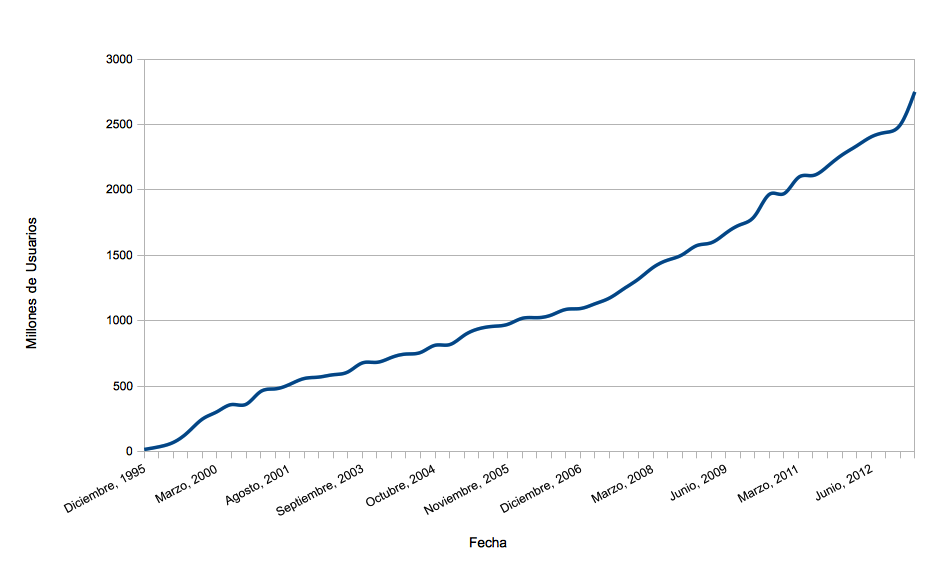
\includegraphics[width=\textwidth]{img/grafCrecInternet}
	\caption{\small Crecimiento de la cantidad de usuarios de Internet, informaci'on extra'ida de \cite{iws}}
	\label{grafCrecInternet}
\end{figure}

Adem'as de la cantidad de usuarios, en paralelo iba creciendo la cantidad de Dominios. En sus inicios, la cantidad de dominios era de 19.732 (medici'on realizada en Agosto de 1995), la medici'on m'as actual (Febrero 2014) realizada por Netcraft\footnote{NetCraft - http://news.netcraft.com/} da un total aproximado de sitios de 920.102.079 \citep{netcraft} (58 millones m'as que el mes anterior). Esto se puede ver en el Gr'afico \ref{grafNetcraft}.

\begin{figure}[h]
  	\centering
	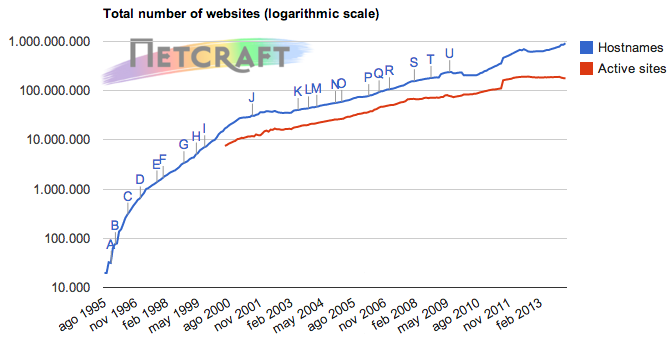
\includegraphics[width=\textwidth]{img/grafNetcraft}
	\caption{\small Crecimiento de la cantidad de sitios en Internet, extra'ido de \cite{netcraft}}
	\label{grafNetcraft}
\end{figure}

Tambi'en fu'e aumentando el tama'no promedio de los sitios as'i tambi'en como la cantidad de recursos que poseen los mismos. En el a'no 1997, el tama'no promedio de un sitio era de 60Kb \citep{atw}, pr'acticamente era todo texto, pocas im'agenes y poca interactividad. Esto fu'e cambiando con el tiempo, con el avance de la tecnolog'ia y de los recursos que se pod'ian compartir en la red. El crecimiento a lo largo del tiempo puede verse en el Gr'afico \ref{grafCrecSitios}

\begin{figure}[h]
  	\centering
	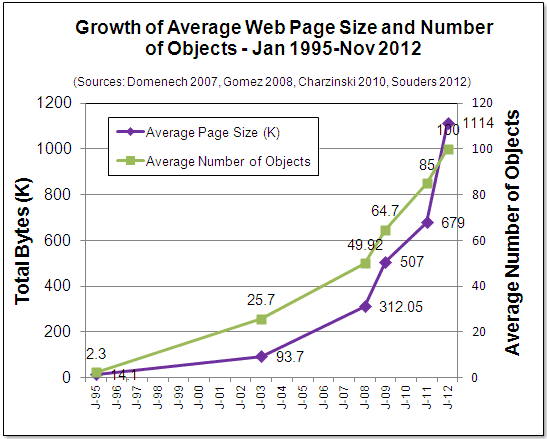
\includegraphics[width=\textwidth]{img/grafCrecSitios}
	\caption{\small Crecimiento del tama'no de los sitios en Internet (1995 a 2012), extra'ido de \cite{tamanoSitios}}
	\label{grafCrecSitios}
\end{figure}

Actualmente, el promedio es de 1687Kb\footnote{Medici'on extra'ida de \citep{httparchive} el 1 de Febrero 2014}, su contenido es mucho m'as variado e interactivo. Hoy los sitios se componen de diversos tipos de recursos, scripts, hojas de estilo, diferentes tipos de im'agenes, video, contenido Flash\footnote{http://www.adobe.com/}, etc. El promedio detallado por contenido de los sitios se pueden ver en el Gr'afico \ref{grafSitiosFeb2014}

\begin{figure}[h]
  	\centering
	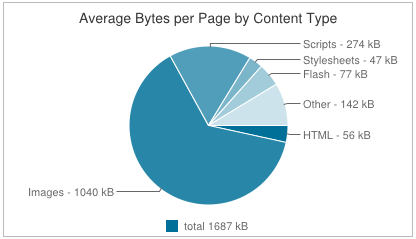
\includegraphics[width=\textwidth]{img/grafSitiosFeb2014}
	\caption{\small Tama'no promedio de los sitios en Internet, detallado por contenido, extra'ido de \cite{httparchive}}
	\label{grafSitiosFeb2014}
\end{figure}


FALTA: UTILIZACION HTTP HTTPS
\chapter{Conceptos sobre Protocolos}
\label{protocolos}
\section{Definici'on}
Un protocolo de comunicaci'on es un conjunto de reglas y normas de transmisi'on, que permite a dos o m'as entidades, comunicarse entre s'i.

\begin{quote}
\textit{''Un protocolo define el formato y el orden de los mensajes intercambiados entre dos o m'as entidades que se comunican, as'i como las acciones que se toman en la transmisi'on y/o recepci'on de un mensaje u otro evento \citep{redesComputadores}.''}
\end{quote}

Es necesario que, antes de establecer una comunicaci'on entre partes, se definan ciertos protocolos para poder asegurar la interoperabilidad y hacer posible la comunicaci'on entre el emisor y receptor.

Las reglas definen la forma en la que debe efectuarse la comunicaci'on, incluyendo cuestiones como la temporizaci'on, secuencia, revisi'on y correcci'on de errores. Define una \textit{sintaxis} (formato de los mensajes), una \textit{sem'antica} (significado de los mensajes) y \textit{sincronizaci'on} (secuenciamiento y temporizaci'on en la comunicaci'on).

Las tareas a realizar se dividen en niveles (capas), luego, los protocolos de cada capa son los que resuelven las tareas. Definir los modelos en capas brinda las siguientes ventajas:

\begin{enumerate}
\item Dividir la comunicaci'on  en partes m'as peque'nas y sencillas
\item Normalizar los componentes de red para permitir el desarrollo y el soporte de los productos de diferentes fabricantes.
\item Permitir la interoperabilidad de diferentes tipos de hardware y software de red para comunicarse entre s'i.
\item Impedir que los cambios en una capa puedan afectar a las otras capas. Facilita la actualizaci'on del protocolo pudiendo modificar un m'odulo a reemplazarlo todo por completo.
\end{enumerate}

\section{Modelo OSI}
\label{osi}
En los inicios de Internet, hubo un gran crecimiento tanto en cantidad como en tama�o de las redes. Debido a esto, muchas de las redes eran incompatibles entre s'i, y era extremadamente complicada la comunicaci'on entre ellas. Para solucionar este problema, la ISO\footnote{International Standard Organization}, realiz'o ciertas investigaciones acerca de los esquemas de red. En 1980 \citep{zim80}, cre'o un modelo de red para ayudar a los dise�adores de redes a poder implementar redes que puedan comunicarse entre s'i y trabajar en conjunto. Este es el modelo de referencia OSI, definida en la ISO/IEC 7498-1 \citep{osi74981}. Este modelo se agrupa en capas, cada capa agrupa una funci'on determinada. Est'an organizadas jer'arquicamente, cada capa ofrece un servicio a la capa superior. Es un modelo te'orico, toma la experiencia de la pila de protocolos TCP/IP (ver \ref{tcpip}), modelo que soporta Internet.

El modelo tiene 7 capas:
\begin{itemize}
\item[7.] Aplicaci'on
\item[6.] Presentaci'on
\item[5.] Sesi'on
\item[4.] Transporte
\item[3.] Red
\item[2.] Enlace
\item[1.] F'isico
\end{itemize}
Se puede ver su distribuci'on en la Figura \ref{capasOSI}

\begin{figure}[h]
  	\centering
	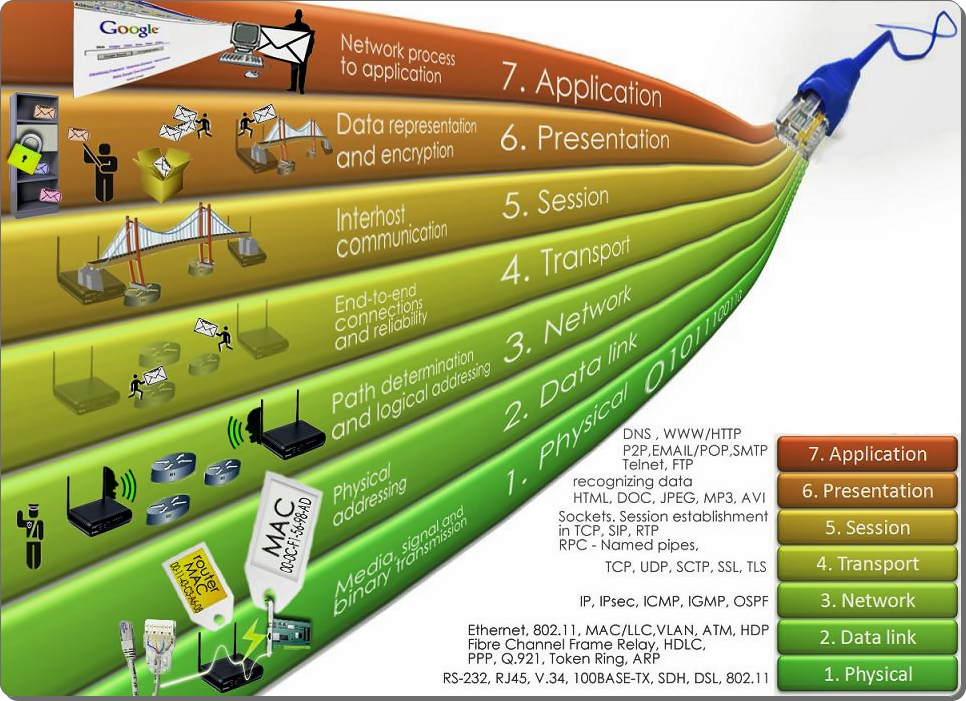
\includegraphics[width=\textwidth]{img/osi}
	\caption{\small Capas OSI, extra'ido de http://www.gargasz.info/}
	\label{capasOSI}
\end{figure}

\subsection{Capa de Aplicaci'on}

Proporciona servicios de red a las aplicaciones del usuario, es la 'unica capa que no provee servicios a otra capa. Si bien es la interfaz hacia el usuario, este no interact'ua directamente con esta capa, sino que lo hace a trav'ez de una aplicaci'on que si tiene acceso directo a esta capa.

\subsection{Capa de Presentaci'on}

Define el formato de los datos que se van a intercambiar entre las aplicaciones y ofrece a los programas de aplicaci'on un conjunto de servicios de transformaci'on de datos. Esta capa es la encargada de manejar las estructuras de datos abstractas y realizar las conversiones de representaci'on de datos necesarias para la correcta interpretaci'on de los mismos.

\subsection{Capa de Sesi'on}

Esta capa establece, administra y finaliza las sesiones entre las partes intervinientes en la comunicaci'on, a esto se le llama Servicio de Administraci'on de la Sesi'on. Tambi'en realiza el control del intercambio de datos y sincroniza el di'alogo entre las partes, a esto se le llama Servicio de Administraci'on del Di'alogo.

\subsection{Capa de Transporte}

Esta capa provee un servicio de transporte universal. Ofrece transparencia en el intercambio de datos entre los hosts involucrados (extremo a extremo) y a'isla a las capas superiores de los detalles de implementaci'on del transporte. Asegura que los datos enviados lleguen en el mismo orden en el que han sido enviados y sin errores, brindando calidad de servicio y confiabilidad en la comunicaci'on.

\subsection{Capa de Red}

Se encarga de la conexi'on de hosts que pueden encontrarse en redes diferentes, define un esquema de direccionamiento, enrutamiento y selecci'on de rutas. Permite que los datos viajen de un extremo a otro a trav'ez de redes interconectadas. Se utilizan los paquetes como unidad de informaci'on, estos paquetes son los que se rutean a trav'ez de la red para llegar del origen al destino.

\subsection{Capa de Enlace}

Proporciona una comunicaci'on confiable entre equipos adyacentes. Se ocupa del direccionamiento f'isico, la topolog'ia de la red y el acceso a la misma. Se utilizan tramas como unidad de informaci'on, aqu'i se realizan los controles de flujo, controles de secuencia, y notificaci'on de errores.

\subsection{Capa F'isica}

Esta capa provee las caracter'isticas procedurales, funcionales, el'ectricas y mec'anicas para establecer, mantener y cerrar conexiones f'isicas. Define como se transmiten los datos al medio, recibe mensajes y los transforma en bits para su posterior env'io a trav'es de se'nales. Ciertas caracter'isticas tales como los conectores f'isicos, niveles de voltaje, duraci'on de un bit, velocidad de los datos f'isicos, temporizaci'on y otros datos similares son definidos por las especificaciones de esta capa.

\subsection{Funciones de los Protocolos}

Entre las funciones de los protocolos se encuentran:
\begin{enumerate}
\item Encapsulamiento: 

Cada capa define lo que se conoce como PDU (Unidad de Datos del Protocolo), que es el resultado de la capa anterior con informaci'on propia. A medida que los datos van bajando a trav'es de las capas se agregan encabezados y eventualmente una cola a los datos con informaci'on correspondiente a cada capa. Estos agregados contienen informaci'on de control para asegurar la entrega de los datos y la correcta interpretaci'on de los mismos en el receptor. Una vez que se re'una la informaci'on de todas las capas, se convierten en bits y son enviadas por el medio f'isico. En la Figura \ref{encapsulamiento} puede verse como se van acoplando las PDUs a medida que se avanza hacia abajo en el Modelo OSI.

\begin{figure}[h]
  	\centering
	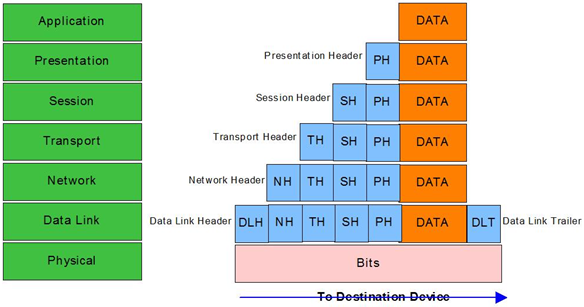
\includegraphics[width=\textwidth]{img/encapsulamiento}
	\caption{\small Encapsulamiento en el Modelo OSI, extra'ida de \cite{encapsulamiento}}
	\label{encapsulamiento}
\end{figure}
\item Establecimiento, control y cierre de la conexi'on.
\item Control de Flujo:
Asegurar que la velocidad de los datos no sature las posibilidades particulares de cada capa.
\item Control de Errores: Detecci'on y correcci'on de errores.
\item Multiplexaci'on: Posibilidad de compartir el canal entre varias conexiones.
\item Encriptaci'on y compresi'on.
\end{enumerate}

\section{TCP/IP}
\label{tcpip}
El conjunto de protocolos TCP/IP permite que computadoras de distintos tama'nos, marcas, y diferentes sistemas operativos puedan lograr una comunicaci'on entre s'i \citep{tcpipIluistrated}. Su desarrollo comenz'o hacia los a'nos 60', y en los 90' se convirtieron en los protocolos m'as utilizados en las redes.
Conforma la base de Internet, la \textsc{wan}\footnote{Wide Area Network, Red de 'Area Amplia} que conecta millones de dispositivos en todo el planeta.

Tiene un dise'no en capas similar al del Modelo OSI (ver Secci'on \ref{osi}), en donde cada capa provee una funcionalidad diferente para la comunicaci'on. El modelo posee 4 capas, Aplicaci'on, Transporte, Red y Enlace, como puede verse en la Figura \ref{tcpip}.

\begin{figure}[ht]
  	\centering
	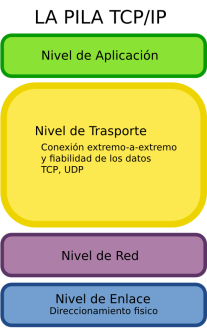
\includegraphics[width=140px]{img/tcpip}
	\caption{\small TCP/IP}
	\label{tcpip}
\end{figure}

\subsection{Las Capas}

\begin{enumerate}
\item Aplicaci'on

En esta capa se manejan los detalles de una aplicaci'on particular. Aqu'i se encuentran protocolos muy conocidos tales como HTTP (Hipertext Transfer Protocol), HTTPS (Hipertext Transfer Protocol Secure),  FTP (File Transfer Protocol), POP (Post Office Protocol), SMTP (Simple Mail Transfer Protocol), SNMP (Simple Network Management Protocol), Telnet (para login remoto), DNS (Domain Name System) \citep{redesComputadores}.
\item Transporte

Provee el servicio de env'io de flujo de datos entre dos hosts. En esta capa se encuentran 2 protocolos muy importantes:

	\subitem TCP (Transfer Control Protocol):
	\label{tcp}
	Permite crear conexiones entre hosts para el env'io de flujos de datos. Se ocupa de dividir los datos que vienen de la capa de aplicaci'on en paquetes de un tama'no adecuado para realizar el env'io en las capas inferiores. Tambi'en se encarga del control de la recepci'on de los paquetes enviados, as'i tambi'en como el establecimiento de los tiempos de espera para asegurarse que el otro extremo reconoce los paquetes enviados. Realiza la multiplexaci'on de la conexi'on, es decir, que permite compartir el canal entre varias conexiones.
	
	Para establecer la conexi'on entre los 2 extremos, el servidor debe dejar en ''escucha'' una direcci'on en un puerto determinado. El cliente, env'ia un mensaje SYN\footnote{SYNchronize} inicial al servidor para iniciar la negociaci'on, el servidor contesta con un paquete SYN-ACK\footnote{ACKnowledgement} que es contestado por el cliente por un ACK. Una vez intercambiados estos 3 mensajes, el cliente puede empezar a realizar las peticiones al servidor. Esto se llama Three Way Handshake (Negociaci'on de 3 v'ias), y puede verse en la Figura \ref{threeway}.
	
	\begin{figure}[ht]
  	\centering
	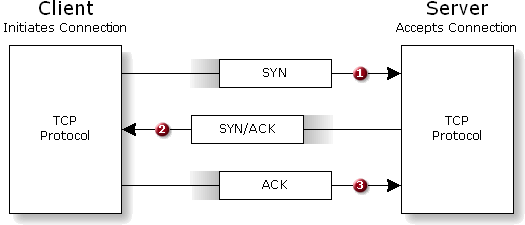
\includegraphics[width=\textwidth]{img/threeway}
	\caption{\small Three Way Handshake, extra'ido de https://www.grc.com/}
	\label{threeway}
	\end{figure}

	\subitem UDP (User Datagram Protocol):
	
	Se ocupa de enviar paquetes de datos llamados datagramas de un extremo a otro, sin realizar una conexi'on previa, el mismo datagrama posee suficiente informaci'on para llegar a destino. No brinda ninguna garant'ia de que el paquete llegue a su destino y tampoco hace control de flujo.
\item Red

Esta capa, a veces llamada capa de Internet, maneja el movimiento de los paquetes a trav'es de la red. El enrutamiento y encaminamiento de los paquetes tiene lugar en esta capa. El protocolo principal de esta capa es IP (Internet Protocol), define el direccionamiento de la capa de red, los campos del datagrama, y las acciones tomadas por los routers y los sistemas finales sobre el datagrama bas'andose en los valores de dichos campos \citep{redesComputadores}. Otros protocolos de esta capa son: ICMP (Internet Control Message Protocol) e IGMP (Internet Group Management Protocol).

\item Enlace

Esta capa, a veces llamada capa de enlace de datos o capa de interfaz de red, incluye el driver\footnote{Controlador de Dispositivo} del sistema operativo y la correspondiente placa de red del dispositivo. Juntos se encargan de todos los detalles del hardware y de la interconexi'on f'isica con el medio (Cable, WiFi, Fibra 'Optica, etc.).
\end{enumerate}

\subsection{TCP/IP y el Modelo OSI}

Similitudes
\begin{enumerate}
\item Ambos se dividen en capas.
\item Ambos tienen Capa de Aplicaci'on, pero ofrecen servicios diferentes.
\item La capa de transporte y la de red son similares.
\item La conmutaci'on es por paquetes\footnote{M'etodo de env'io de datos, cada paquete posee datos e informaci'on de control que indica la ruta a destino.} (no por circuitos).
\end{enumerate}

Diferencias:
\begin{enumerate}
\item En la capa de aplicaci'on de TCP/IP se combinan las capas de presentaci'on y de sesi'on del Modelo OSI.
\item En la capa de enlace de TCP/IP se combinan las capas de enlace y de f'isica del Modelo OSI.
\item Al tener menos capas, TCP/IP es m'as simple.
\item TCP/IP es el est'andar de Internet, las redes no se desarrollan a partir del Modelo OSI, se utiliza como gu'ia.
\end{enumerate}

\begin{figure}[h]
  	\centering
	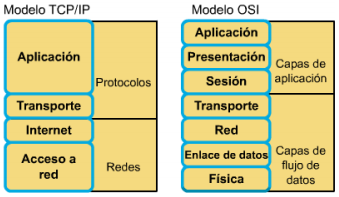
\includegraphics{img/tcpiposi}
	\caption{\small Comparaci'on entre TCP/IP y OSI}
	\label{tcpiposi}
\end{figure}

\section{HTTP}
\label{http}
Las siglas de este protocolo son por HyperText Transfer Protocol (Protocolo de Transferencia de Hipertexto). Es un protocolo de capa de aplicaci'on (ver Secci'on \ref{osi}) que sirve para distribuir informaci'on. Fu'e utilizado en la web desde el a'no 1990 en su primera versi'on (0.9), en la que simplemente se pod'ia transferir texto plano. Su evoluci'on fue el est'andar 1.0 en el que se mejor'o el protocolo permitiendo que los mensajes usen el formato \gls{mime}, se incorporaron metadatos acerca de la informaci'on transferida y modificadores en la sem'antica de petici'on/respuesta. La revisi'on del protocolo que se usa actualmente es la 1.1, definida en la RFC 2616 \citep{rfcHTTP1.1}. Contiene nuevos metodos, headers y otras caracter'isticas. Las principales diferencias de esta 'ultima definici'on se pueden ver en \citep{http1011}.

El contenido web reside en servidores, estos son los que se comunican utilizando este protocolo entre otros. Sirven \textsc{recursos}, estos recursos pueden ser p'aginas HTML, im'agenes, PDF's, video, etc, tanto contenido est'atico como din'amico (generado a demanda). Debido a la gran diversidad de contenido que provee un Servidor, es necesario identificar el tipo de recurso que se est'a enviando. Esto se hace utilizando una etiqueta llamada MIME-Type, que define el tipo de contenido a transferir.

Cada recurso del servidor tiene un nombre, para que los clientes puedan apuntar directamente al recurso deseado. Se nombra con una URL, que tiene el siguiente formato:

\begin{quote}
PROTOCOLO://SERVIDOR/PATH\_AL\_RECURSO/RECURSO
\end{quote}

El funcionamiento b'asico es, el cliente env'ia una petici'on al servidor (al puerto 80 por defecto) y este le responde. Esta comunicaci'on se realiza a trav'es de mensajes HTTP. Existen diferentes m'etodos que se pueden utilizar cuando se env'ia una petici'on al servidor, tales como

\begin{enumerate}
\item GET - El cliente solicita un recurso espec'ifico del servidor.
\item POST - El cliente env'ia datos que van a ser utilizados por el servidor.
\item HEAD - El cliente solicita s'olo los Headers (se detallar'an m'as adelante).
\end{enumerate}

Estos son algunos de los m'etodos, hay otros tales como PUT, DELETE, etc. Seg'un el m'etodo, el servidor opera de manera diferente. En la petici'on se env'ia el m'etodo, el recurso solicitado, la versi'on del protocolo utilizado, el host, el user-agent\footnote{Qui'en est'a generando la petici'on, por ejemplo Mozilla, Safari, Squid (browser, proxy, etc.).}, entre otros.
El servidor, responde a la petici'on con una respuesta, que contiene un c'odigo de estado de 3 d'igitos que le dice al cliente que la petici'on fue exitosa u otras, por ejemplo 200 (OK) o 404 (Documento no encontrado) de los m'as comunes.

Los mensajes de HTTP consisten en peticiones y respuestas, sus formatos son similares. Consisten en 3 partes:

\begin{enumerate}
\item Linea Inicial - Se indica que hacer en la petici'on o que fue lo que pas'o en la respuesta.
\item Headers - Ac'a se pueden definir diferentes par'ametros por c'ada l'inea con la sintaxis ''nombre:valor''.
\item Cuerpo - Esta parte contiene los datos enviados, ya sea del cliente al servidor o viceversa.
\end{enumerate}

El formato de una petici'on es el siguiente:

\begin{quote}
$<$m'etodo$>$ $<$url del recurso$>$ $<$versi'on$>$

$<$headers$>$

$<$cuerpo$>$
\end{quote}

El formato de la respuesta es el siguiente:

\begin{quote}
$<$versi'on$>$ $<$estado$>$ $<$descripci'on del estado$>$

$<$headers$>$

$<$cuerpo$>$
\end{quote}

\subsection{HEADERS}
\label{headers}
Los headers, a'naden informacion adicional a las peticiones y respuestas. El protocolo define varios headers, pero se pueden inventar tambi'en, los servidores y clientes son libres de hacerlo. Hay diferentes tipos de headers, entre los que se encuentran:

\begin{enumerate}
\item Headers generales

Pueden aparecer en peticiones y respuestas.
\item Headers de peticiones.

Proveen m'as informaci'on acerca de las peticiones.
\item Headers de respuesta.

Proveen informaci'on acerca del recurso del mensaje.
\item Headers de extensi'on

Permite agregar nuevos headers que no est'en dentro de la especificaci'on est'andar \citep{rfcHTTP1.1}.
\end{enumerate}

La definici'on completa de los headers se encuentra en la Secci'on 14 de \citep{rfcHTTP1.1}.

\section{HTTPS}

Los usuarios de Internet, utilizan la web para hacer transacciones que requieren que el nivel de seguridad sea fuerte. Operaciones como realizar transacciones bancarias o hacer compras online, no se realizar'ian si los datos que el usuario env'ia al servidor viajan desprotegidos. Ante esta necesidad, se combina el protocolo HTTP con la tecnolog'ia de encriptaci'on digital.
HTTPS es la versi'on ''segura'' de HTTP, a'nade a este protocolo, una capa de cifrado utilizando SSL \footnote{Secure Sockets Layer.} (el predecesor de TLS\footnote{Transport Layer Security.}) sobre TCP, como se puede ver en la Figura \ref{httpvshttps}. Se define en la RFC 2818 \citep{rfcHTTPS}. Se distingue el tr'afico seguro del inseguro por la utilizaci'on de un n'umero de puerto diferente.

\begin{figure}[h]
  	\centering
	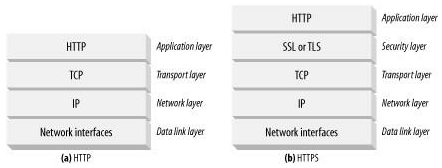
\includegraphics{img/httpvshttps}
	\caption{\small Comparaci'on entre HTTP y HTTPS, extra'ido de \citep{httpGuide}}
	\label{httpvshttps}
\end{figure}

Permite que los datos que viajan entre cliente y servidor vayan encriptados, esto se hace antes de enviar los datos por la red. Se distingue f'acilmente porque el formato de la URL empieza con https:// y la conexi'on por defecto se establece con el puerto 443. Es decir, si el browser hace una petici'on a un servidor, en la cual, el esquema es https, se inicia la negociaci'on para establecer la conexi'on segura con el mismo.

La conexi'on se hace con otro puerto diferente al de HTTP ya que SSL es un protocolo binario, completamente diferente. Si ambos llegaran al mismo puerto, los servidores interpretarian SSL como HTTP err'oneo y cerrar'ian la conexi'on.

\subsection{Criptograf'ia}

La criptograf'ia es el arte y la ciencia de codificar y decodificar mensajes, alterando la representaci'on lingu'istica de mensajes, buscando la confidencialidad y para prevenir la manipulaci'on de los mismos. Tambi'en se utiliza para probar quien fue el autor del mensaje o una transacci'on (no repudio).

Se basa en Algoritmos de Cifrado (Ciphers) que tienen un m'etodo para codificar el mensaje y otro para decodificarlo posteriormente. Comenzaron siendo algoritmos simples hasta que se empezaron a construir m'aquinas\footnote{Ver M'aquina Enigma Alemana, http://www.bbc.co.uk/history/topics/enigma} para reforzar la seguridad de la encriptaci'on haciendo operaciones m'as complejas. A causa de que estos algoritmos y m'aquinas pod'ian llegar a manos no apropiadas, se incluyeron diversos m'etodos (llaves met'alicas, diales de configuraci'on), que actuan como entrada para que el algoritmo o m'aquina pudiera funcionar. De esta manera, a'un teniendo el algoritmo o dispositivo, sin la clave no se puede decodificar.

En la era digital, los m'etodos (clave) para la entrada de los algoritmos de encriptaci'on son simplemente n'umeros. Estos algoritmos son funciones que toman una porci'on de datos y la codifican/decodifican basados en el algoritmo de encriptaci'on y la clave proporcionada.

\subsubsection{Criptograf'ia Sim'etrica}

La criptograf'ia puede ser sim'etrica, es decir, que la clave para encriptar y desencriptar el mensaje es la misma. De esta manera, tanto el emisor como el receptor deben intercambiarse previamente la clave, antes de comenzar la comunicaci'on.

El algoritmo m'as conocido de criptograf'ia sim'etrica es el DES (Data Encryption Standard) \citep{des}. Se trata de un algoritmo que utiliza claves de 56 bits para cifrar/descifrar bloques de datos de 64 bits. El uso de m'ultiples claves conduce al algoritmo Triple-DES, en el que DES se aplica 3 veces, consiste en 3 claves de 56 bits que se utilizan sucesivamente en los datos a cifrar/descifrar como puede verse en la Figura \ref{tripleDes}.

\begin{figure}[h]
  	\centering
	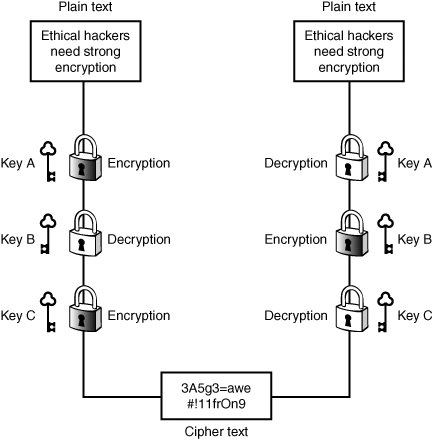
\includegraphics[width=300px]{img/tripleDes}
	\caption{\small Algoritmo Triple-DES, extra'ido de http://flylib.com/}
	\label{tripleDes}
\end{figure}

\subsubsection{Criptograf'ia As'imetrica}

En la criptograf'ia de clave p'ublica (ver Figura \ref{clavePublica}), las claves son Asim'etricas, es decir, que la clave para encriptar difiere de la clave para desencriptar el mensaje. En este tipo de criptograf'ia, la clave para encriptar el mensaje es p'ublica, cualquiera que quiera establecer una conexi'on con seguridad, puede obtener la clave\footnote{Almacenada en servidores de acceso p'ublico.} para iniciar la comunicaci'on. Por otro lado, la clave para desencriptar los mensajes es privada, pertenece al servidor que es el 'unico que puede decodificar los mensajes recibidos por el cliente.

\begin{figure}[h]
  	\centering
	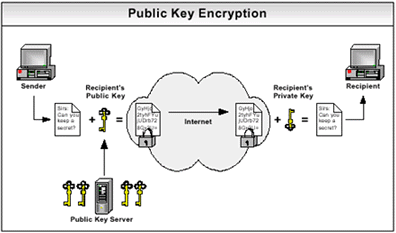
\includegraphics[width=300px]{img/clavePublica}
	\caption{\small Criptograf'ia de Clave P'ublica, extra'ido de http://www.novell.com/}
	\label{clavePublica}
\end{figure}

RSA (Rivest, Shamir y Adleman) \citep{rsa} es un algoritmo asim'etrico que se utiliza en firma digital\footnote{Mecanismo criptogr'afico que permite al receptor del mensaje poder determinar la entidad del emisor y confirmar que el mensaje no ha sido alterado desde que fue firmado.}. La clave utilizada para cifrar es diferente (pero relacionada) a la que se utiliza para descifrar. El algoritmo consta de los siguientes pasos:

\begin{enumerate}
\item Se seleccionan 2 n'umeros primos \textit{p} y \textit{q}.
\item Se calcula el producto de ambos n'umeros \textit{n = p * q}, este n'umero se llama \textit{m'odulo}.
\item Se elige un n'umero entero \textit{e} tal que \textit{1 $<$ e $<$ (p-1)*(q-1)}.
\item Se calcula \textit{d = $e^{-1}$ mod[(p-1)*(q-1)]}.
\end{enumerate}
La clave p'ublica es el par de n'umeros (n,e) y la clave privada es el par de n'umeros (n,d).

Para encriptar un mensaje \textit{m} se calcula:
\begin{quote}
$c \equiv m^e \pmod{n}$
\end{quote}
Para desencriptar un mensaje \textit{c} se calcula:
\begin{quote}
$\equiv c^d \pmod{n}$
\end{quote}

\subsection{Conexi'on}

Una conexi'on es el enlace que se establece entre el emisor y el receptor a trav'es del cual, se env'ia un mensaje. El procedimiento para iniciar una comunicaci'on HTTPS es el siguiente: El cliente abre una conexi'on con el puerto 443 al servidor. Una vez que la conexi'on TCP est'a establecida, el cliente y el servidor inicializan la capa SSL negociando algunos par'ametros criptogr'aficos e intercambiando llaves. Una vez concluida esta negociaci'on, ya pueden empezar a intercambiar mensajes encriptados. Se puede ver en detalle en la Figura \ref{httpsConnection}.

\begin{figure}[h!]
  	\centering
	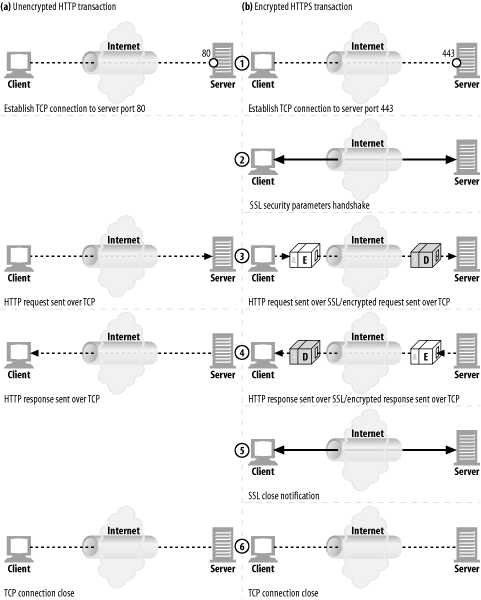
\includegraphics[width=390px]{img/httpsConnection}
	\caption{\small Establecimiento de Conexiones HTTP y HTTPS, extra'ido de \citep{httpGuide}}
	\label{httpsConnection}
\end{figure}

\section{SPDY}
\label{spdy}

\subsection{Introducci'on}

SPDY es un protocolo experimental desarrollado por Google a mediados del 2009, cuya meta principal es reducir los tiempos de carga de los sitios enfoc'andose en las limitaciones de HTTP (ver \ref{http}).
Espec'ificamente se busca lo siguiente \citep{highPerformance}:
\begin{enumerate}
\item Reducir el Tiempo de Carga de los Sitios.
\item Evitar la necesidad de que los desarrolladores tengan que realizar cambios a los sitios actuales.
\item Evitar cambios en la infraestructura de las redes y minificar la complejidad de implementaci'on.
\item Liberar el desarrollo a la comunidad de c'odigo abierto.
\item Recopilar datos reales de rendimiento para validar o invalidar el protoclo experimental.
\end{enumerate}
Desde el a'no 2012 el protocolo es soportado por los navegadores Chrome\footnote{http://www.google.com/intl/es\_AR/chrome/browser/}, Mozilla Firefox\footnote{http://www.mozilla.org/es-AR/firefox/new/}, y Opera\footnote{http://www.opera.com/}. Existen varias opciones de servidores que soportan el protocolo tales como Apache\footnote{http://code.google.com/p/mod-spdy/}, Jetty\footnote{http://wiki.eclipse.org/Jetty/Feature/SPDY} y NodeJS\footnote{https://github.com/indutny/node-spdy}. Varios sitios populares (Google, Facebook, Twitter) ya ofrecen un cliente para la utilizaci'on del protocolo. 

\subsection{Detalles del Protocolo}

Es un protocolo que a'nade una capa de sesi'on que funciona sobre SSL (ver Figura \ref{capaSPDY}) que permite la transmisi'on de m'ultiples Streams\footnote{Flujo de Datos.} sobre una conexi'on TCP. Especifica un nuevo formato de trama para codificar y transmitir datos.
Su especificaci'on se puede ver en \citep{spdyWhitepaper} y su draft se puede encontrar en \citep{spdyDraft}.

\begin{figure}[h]
  	\centering
	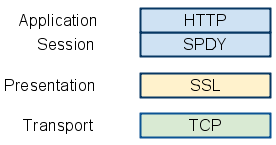
\includegraphics[width=200px]{img/capaSPDY}
	\caption{\small Protocolo de Aplicaci'on SPDY, extra'ido de \citep{spdyWhitepaper}}
	\label{capaSPDY}
\end{figure}

El protocolo HTTP no tiene estado, y, por cada recurso que requiera existe la necesidad de abrir una conexi'on nueva y cerrarla. Esto trae varios problemas:
\begin{enumerate}
\item Por cada conexi'on nueva que se hace, se necesitan varios mensajes para establecer la conexi'on TCP, lo que trae varios RTT (Round Trip Time) adicionales a la comunicaci'on. El RTT es el tiempo estimado para enviar y recibir un mensaje por parte del interlocutor \citep{tcpipIluistrated}, puede verse en la Figura \ref{rtt}.

\begin{figure}[h]
  	\centering
	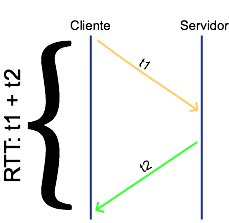
\includegraphics[width=200px]{img/rtt}
	\caption{\small RTT}
	\label{rtt}
\end{figure}

\item Retrasos debido al ''Slow Start'' de TCP. Se comienza enviando un volumen de datos peque'no hasta alcanzar cierto valor llamado Umbral de Congesti'on.
\item Clientes que evitan realizar m'ultiples conexiones con el mismo servidor (hasta 6 actualmente).
\item  A su vez, los servidores crean varios subdominios para almacenar el contenido para que los clientes puedan realizar las peticiones sin tener que evitar las m'ultiples conexiones a un mismo dominio.
\end{enumerate}

El funcionamiento b'asico de SPDY \ref{spdy} puede verse en la Figura \ref{spdy}. Inicia la conexi'on con el servidor realizando el ThreeWay Handshake de TCP (ver \ref{tcp}), se establece una conexi'on segura entre ambos extremos, y luego se pueden empezar a pedir los recursos a trav'es de la misma conexi'on y en paralelo.
%\clearpage
\begin{figure}[ht!]
  	\centering
	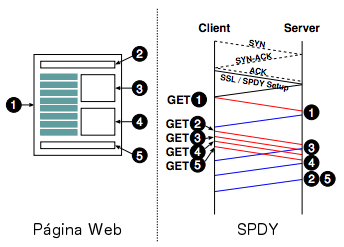
\includegraphics[width=230px]{img/spdy}
	\caption{\small Funcionamiento de SPDY, extra'ido de \citep{towards}}
	\label{spdy}
\end{figure}

SPDY ofrece por sobre HTTP las siguientes mejoras:
\begin{enumerate}
\item Peticiones Multiplexadas. No existen l'imites de peticiones que se pueden realizar en una sesi'on de SPDY. A causa de que las peticiones son multiplexadas aumenta la eficiencia del protocolo TCP.
\item Priorizaci'on de Peticiones. Los clientes pueden solicitar al servidor cu'ales recursos quiere obtener antes que otros. Esto evita la congesti'on de recursos que no son cr'iticos cuando todav'ia est'a pendiente el env'io de alg'un recurso que tiene una prioridad mayor.
\item Compresi'on de Headers. A causa de que hoy en d'ia los clientes env'ian mucha informaci'on redundante en forma de Headers, como la cantidad de peticiones para obtener un sitio promedio va desde 50 a 100, esta cantidad de informaci'on es relevante. Comprimir los Headers reduce el ancho de banda utilizado.
\item Server Push. Al permitir la comunicaci'on bi-direccional a trav'es de streams, cualquiera de los 2 (cliente o servidor) puede iniciar un stream hacia el otro. El servidor puede enviar un recurso al cliente antes de que este lo pida\footnote{El servidor conoce de antemano que el cliente va a necesitar el recurso en cuesti'on.}, esto reduce el tiempo de carga del sitio y disminuye la cantidad de peticiones del cliente.
\item Server Hint. El servidor puede ''sugerirle'' al cliente que pida un recurso en particular, ya que lo va a necesitar. De todas maneras, el servidor espera a que el cliente peticione el recurso en cuesti'on antes de enviarlo. Esto reduce el tiempo que tarda el cliente en descubrir cuales son los recursos que tiene que pedirle al servidor.
\end{enumerate}

SPDY se enfoca en la manera en la que se transmiten los datos por la red, preserva toda la sem'antica del protocolo HTTP. De esta manera, para las aplicaciones se implementa de manera transparente, ya que reside entre la capa de aplicaci'on y la de transporte. Esta sesi'on es similar al par petici'on-respuesta de HTTP. Es obligatoria la compresi'on del mensaje.

\subsection{Alternativas Propuestas}

Existen varias alternativas que se propusieron para mejorar la performance de Internet, 

\subsubsection{SCTP (Stream Control Transmission Protocol)}
Es una alternativa al Protocolo TCP, definido en la RFC 2960 \citep{rfcSCTP}, provee confiabilidad, control de flujo y secuenciaci'on, opcionalmente permite el env'io de mensajes sin un orden preestablecido. Permite Multihoming, que es la capacidad de que los extremos conectados puedan tener m'as de una direcci'on IP.

\subsubsection{HTTP sobre SCTP}

Es una propuesta de utilizar HTTP sobre SCTP definida en el draft ''draft-natarajan-http-over-sctp-00'' \citep{sctpHTTP}. El servicio de m'ultiples streams de SCTP es la caracter'istica que beneficia la combinaci'on de protocolos. Las transacciones HTTP independientes cuando se transmiten sobre diferentes streams de SCTP mejoran significativamente los tiempos de respuesta.

\subsubsection{Structured Stream Transport (SST)}

Es un protocolo de transporte experimental \citep{sst} dise'nado para las aplicaciones que requieren de muchas conexiones as'incronas en paralelo, tales como la descarga de las diferentes partes que componen un sitio web y reproducir simult'aneamente m'ultiples flujos de audio y video a la vez.
No realiza el 3-way Handshake en el inicio como TCP. Multiplexa flujos de datos de aplicaciones en una sola conexi'on de red. Soporta mensajes/datagramas de cualquier tama'no, no hay necesidad de limitar el tama'no de los env'ios. Priorizaci'on de flujos de datos.
\subsubsection{MUX y SMUX}

MUX\footnote{http://www.w3.org/Protocols/MUX/} y SMUX\footnote{http://www.w3.org/TR/WD-mux} son protocolos de capa intermedia (entre la capa de transporte y la capa de aplicaci'on) que proporcionan la multiplexaci'on de flujos de datos. Se propusieron al mismo tiempo que HTTP/1.1.

\subsection{Estudios Relacionados}
\label{estudiosSPDY}
Se han realizado diversos estudios acerca de la performance de SPDY, que arrojan diferentes resultados. Estos resultados ayudan a ver en qu'e condiciones la utilizaci'on de SPDY realmente mejora la performance de la carga de un sitio.

Jitendra Padhye y Henrik Frystyk Nielsen, en su paper ''A comparison of SPDY and HTTP performance'' \citep{comparision}, realizaron una comparaci'on de ambos protocolos en un ambiente controlado. Con un sitio de prueba\footnote{index.html + 20 im'agenes + 3 hojas de estilo}, variando el RTT y el ancho de banda, obtuvieron los resultados que se ven en los Gr'aficos \ref{comparision1} y \ref{comparision1}.

\begin{figure}[ht!]
  	\centering
	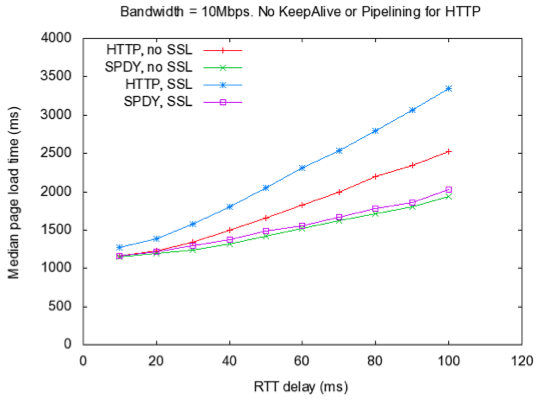
\includegraphics[width=230px]{img/comparision1}
	\caption{\small SPDY vs HTTP - 10Mbps, extra'ido de \citep{spdyWhitepaper}}
	\label{comparision1}
\end{figure}

\begin{figure}[ht!]
  	\centering
	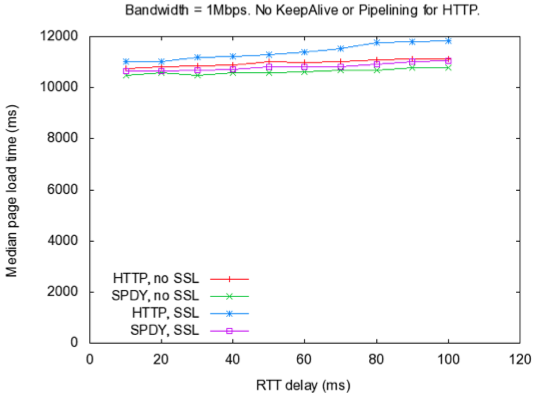
\includegraphics[width=230px]{img/comparision2}
	\caption{\small SPDY vs HTTP - 1Mbps, extra'ido de \citep{spdyWhitepaper}}
	\label{comparision2}
\end{figure}

Claramente se observa que, con anchos de banda m'as limitados, el incremento de performance de SPDY es bajo (del 3\% al 8\%) frente a un ancho de banda de 10mb en el cual el incremento es de hasta 39\%. Lo cual es un indicador de que, en un ambiente en el cual la velocidad del enlace sea pobre (por ejemplo una red 3G), que causa que est'e sujeto a una mayor probabilidad de p'erdidas de paquetes, SPDY no funciona como lo esperado. Posiblemente a causa del alto costo de retransmisi'on del flujo de datos, ya que si el Stream se pierde, se debe retransmitir todo completo ya que usa una sola conexi'on entre los extremos para comunicarse.

Otro estudio interesante, relacionado con los resultados del estudio anterior, es ''Towards a SPDYier Mobile Web?'' \citep{towards}. En este paper se estudi'o el rendimiento de SPDY vs HTTP en redes de celulares. Tambi'en concluyen que no hay una diferencia significativa entre los protocolos estudiados en ese ambiente en particular.

\vspace{5mm}

FALTAN

The Effect of Network and Infrastructural Variables on SPDY?s Performance

How Speedy is SPDY?
\chapter{Problem'aticas asociadas a la Web}
\label{problematica}

\section{Introducci'on}

Debido al crecimiento de Internet visto en el C'apitulo \ref{desarrolloWeb} y a los problemas que presenta el protocolo HTTP en su implementaci'on (visto en el C'apitulo \ref{protocolos}), mejorar los tiempos de carga de los sitios web es clave.

VER http://munchweb.com/effect-of-website-speed

\section{Performance}

Cada aplicaci'on se desarrolla con los requerimientos del modelo de negocio, el contexto, las expectativas de los usuarios y la complejidad de la tarea. A causa de esto, hay que planificar y dise'nar, centr'andose en el usuario, y su percepci'on del tiempo de procesamiento \citep{highPerformance}.
Nuestros tiempos de reacci'on son constantes, independientemente del tipo de aplicaci'on o dispositivo utilizado, puede verse en la tabla siguiente:

\begin{quote}
\begin{center}
\begin{tabular}{l | l}
  Retardo & Percepci'on del Usuario \\
  \hline
  0-100ms & Instant'anea \\
  100-300ms & Retraso peque'no perceptible \\
  300-1000ms & La m'aquina se encuentra procesando\\
  1,000+ ms & Distracci'on en lo que se est'a realizando\\
  10,000+ ms & La tarea es abandonada\\
\end{tabular}

Percepci'on del usuario ante los retardos, extra'ido de \citep{highPerformance}.
\end{center}
\end{quote}

Para que la experiencia del usuario sea positiva, el sitio debe renderizarse, o al menos tener una respuesta visual de que el sitio se est'a cargando, en al menos 250 milisegundos.

En agosto del 2010, Mike Belsche\footnote{Ingeniero de Software, fu'e uno de los desarrolladores del protocolo SPDY (ver Secci'on \ref{spdy}) - https://www.belshe.com} public'o un estudio \citep{moreBand} acerca de 2 factores importantes en el Tiempo de Carga de los Sitios, Ancho de Banda y RTT. El RTT\footnote{Round Trip Time} es el tiempo que demora un paquete en ir del emisor al receptor y volver al emisor nuevamente.
Realiz'o 2 experimentos, el primero variando el Ancho de Banda y el segundo variando el RTT.

En el Gr'afico \ref{belshePLTxBW} puede observarse el resultado del primer experimento, al aumentar el Ancho de Banda hay mejoras en el tiempo de respuesta en los valores m'as bajos, pero, a partir de cierto ancho de banda, el aumento no produce mejoras en el rendimiento.

\begin{figure}[ht]
	\begin{center}
	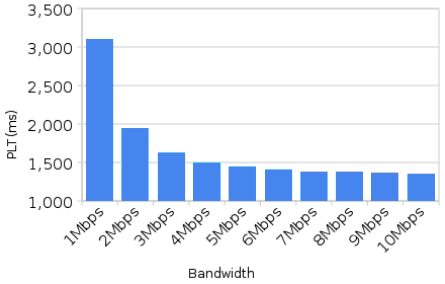
\includegraphics[width=300px]{img/belshePLTxBW}
	\caption{\small Latencia por Ancho de Banda, extra'ido de \citep{moreBand}}
	\end{center}
	\label{belshePLTxBW}
\end{figure}

En cambio, en el Gr'afico \ref{belshePLTxRTT}, se ve claramente que a medida que el RTT se va reduciendo, tambi'ien lo hace el Tiempo de Carga del Sitio, incluso cuando ya el RTT es bajo.

\begin{figure}[ht]
	\begin{center}
	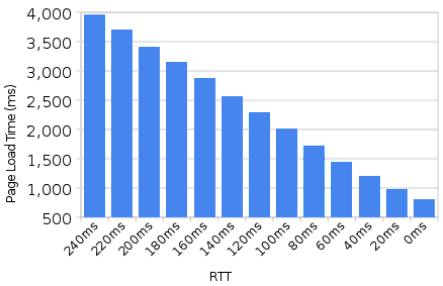
\includegraphics[width=300px]{img/belshePLTxRTT}
	\caption{\small Tiempo de Carga de un sitio a medida que el RTT se decrementa, extra'ido de \citep{moreBand}}
	\end{center}
	\label{belshePLTxRTT}
\end{figure}

La conclusi'on del estudio de Belshe es que, si se duplica su Ancho de Banda sin reducir el RTT significantemente, s'olo se obtiene una mejora m'inima en la Navegaci'on. Disminuir el RTT, sin importar el Ancho de Banda utilizado, siempre supone una mejora en la velocidad. Para acelerar Internet, o bien hay que ocuparse de reducir el RTT, o reducir la cantidad de RTT's requeridos para cargar un sitio.

Es importante tambi'en conocer, d'onde es que el usuario pasa el tiempo esperando en la carga de un sitio web. Seg'un el estudio de Steve Souders en su libro \citep{highPerformanceWebSites}, el cliente tarda menos del 20\% para obtener el documento HTML, y el tiempo restante para recibir el resto de los componentes del sitio. Es importante enfocarse en el 80\%, 90\% restante, ya que el tiempo no se desperdicia en descargar el documento HTML ni en el procesamiento que realiza el servidor antes de enviarnos la petici'on. Esto se resume en la ''Regla de Oro de la Performance'' de dicho libro:

\begin{quote}

\textit{Solo el 10-20\% del tiempo de respuesta del usuario es consumido descargando el documento HTML. El otro 80-90\% se consume descargando todos los componentes de la p'agina.}

\end{quote}

\section{T'ecnicas de optimizaci'on}

Souders, plantea 14 reglas para la optimizaci'on de los sitios que se describen a continuaci'on.

\begin{enumerate}

\item \textbf{Minimizar la cantidad de peticiones.}

La idea b'asica es eliminar las peticiones al servidor, esto se hace utilizando varias t'ecnicas enumeradas a continuaci'on.

	\begin{enumerate}
	\item Mapa de Im'agenes - Permite asociar m'ultiples 'areas en una imagen para que se puedan cliquear y realizar cierta acci'on (el ejemplo m'as b'asico es el de navegar un hiperv'inculo). En vez de utilizar m'ultiples im'agenes para realizar un men'u por ejemplo, se utilizar'ia una sola mapeada. De esta manera se ahorran las peticiones de las im'agenes por 1 sola petici'on.
	\item CSS Sprites - Permite combinar v'arias im'agenes en una sola, luego en el sitio, se define que parte de la imagen combinada desea mostrarse. Por ejemplo, en el sitio de Google cuando se realiza una b'usqueda, se utiliza el Sprite que se ve en la Figura \ref{css_sprites}.
		\begin{figure}[htbp]
		\begin{center}
			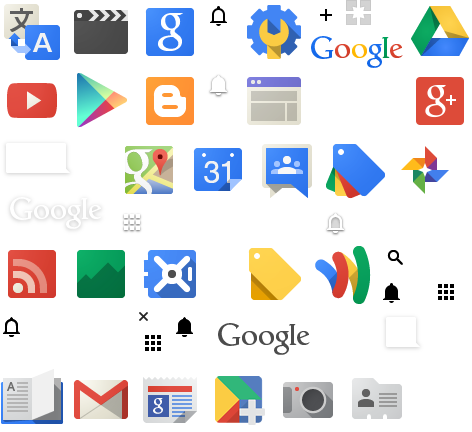
\includegraphics[width=150px]{img/css_sprites}
			\caption{\small Sprite del sitio www.google.com}
		\end{center}
		\label{css_sprites}
		\end{figure}

	A simple vista se ven 44 im'agenes combinadas. La utilizaci'on de este Sprite reducir'ia todas estas peticiones a 1 sola.
	\item Im'agenes Inline - Se pueden incluir im'agenes en un sitio web sin necesidad de realizar una petici'on al servidor definiendolas con el esquema \textit{data:} \ref{rfcData} dentro del c'odigo HTML de la p'agina.
	\item Combinar Scripts y Hojas de Estilo - Como la mayor'ia de los sitios actuales utilizan Javascript y CSS, es preferible que los Scripts se combinen en uno solo al igual que las Hojas de Estilo. En el caso de tener varios archivos, el navegador va a generar una petici'on por cada uno de ellos de no tenerlo almacenado en una copia local.
	\end{enumerate}
\item \textbf{Utilizar un CDN}

La proximidad del cliente al servidor web tiene un impacto en el tiempo de respuesta de las peticiones. No es lo mismo solicitar un recurso localizado China estando en Argentina que uno ubicado dentro del mismo pa'is. Por ende, si los contenidos est'an cerca\footnote{En t'erminos de distancia f'isica.} el tiempo de respuesta es menor. Debido a que solo el 10-20\% del tiempo de respuesta se dedica al HTML (visto al inicio de este cap'itulo), si el resto de los recursos del sitio se encuentran cerca del cliente, se mejorar'ian los tiempos de respuesta. Para esto es necesario dispersar estos recursos geogr'aficamente.

Un CDN\footnote{Content Delivery Networks} es una red de distribuci'on de contenidos. Son servidores dispersados geogr'aficamente que ofrecen r'eplicas de los recursos de un sitio particular para brindarlos al cliente desde el m'as cercano a su locaci'on.

Utilizar el servicio que brinda un CDN mejora los tiempos de respuesta de los usuarios.
\item \textbf{A'nadir Headers para Cach'es}

Cuando un usuario visita el sitio por primera vez, realiza tantas peticiones HTTP como recursos tenga la p'agina. Utilizando Headers Expires o Cache-Control\footnote{Desde HTTP 1.1} (Cap'itulo \ref{protocolos}, Secci'on \ref{headers}) se puede hacer que los recursos puedan ser almacenados en Cach'es (Cap'itulo \ref{cache}). Esto disminuye la cantidad de peticiones en una posterior visita a la p'agina del mismo usuario.

La performance del tiempo de respuesta del sitio mejora seg'un la cantidad de ''Hits''\footnote{Necesidad de solicitar un recurso que ya tengo almacenado en la Cach'e} que el usuario tenga de los componentes del sitio.
\item \textbf{Comprimir los componentes (Gzip)}

Se puede reducir el tiempo de respuesta, disminuyendo el tama'no de la respuesta HTTP. Esto se puede realizar comprimiendo el recurso que se est'a solicitando. La reducci'on del tiempo es mayor en ambientes en donde el ancho de banda es bajo. El formato \textit{Gzip}\footnote{http://www.gzip.org/} \citep{rfcGzip} es el m'as popular y el m'as efectivo, el otro formato que se usa con menos frecuencia es \textit{deflate} \citep{rfcDeflate}.

El usuario tiene que enviar en la petici'on un Header \textit{Accept-Encoding} indicando los m'etodos aceptados. Cuando el servidor recibe este Header, puede comprimir el recurso utilizando alguno de los m'etodos indicados por el usuario. Este devuelve la respuesta con un Header \textit{Content-Encoding} indicando el tipo de compresi'on utilizado en el recurso que se est'a enviando.

Los tipos de archivos que se deber'ian comprimir son aquellos de texto, tales como HTML, Scripts, CSS, etc. Aquellos formatos que ya se encuentran comprimidos como las im'agenes o los archivos PDF no deber'ian comprimirse ya que se desperdicia tiempo de CPU del servidor\footnote{Para realizar la compresi'on.} y adem'as puede incluso incrementar el tama'no del archivo.

\item \textbf{CSS en la parte superior del HTML}

Las Hojas de Estilo deben incluirse en la parte superior del HTML. De esta manera, los navegadores pueden ir renderizando la p'agina a medida que van llegando las respuestas de las peticiones. Esto es importante en t'erminos de usabilidad, para brindarle un medio visual \footnote{Carga progresiva del sitio.} al usuario que est'a esperando el sitio.
\item \textbf{Scripts en la parte inferior del HTML}

Cuando se realizan las peticiones al servidor, las descargas pueden hacerse en paralelo con ciertos l'imites\footnote{2 seg'un la especificaci'on HTTP 1.1, hasta 6 seg'un el navegador}, eso claramente es beneficioso, ya que al paralelizar las descargas, el tiempo es menor comparado con descargas secuenciales. En el caso de los Scripts, esta caracter'istica se deshabilita por 2 motivos,    uno es que si es script altera contenido de la p'agina, el navegador debe esperar a recibirlo para mostrar el contenido correctamente. El otro motivo es que el navegador debe respetar el orden de ejecuci'on de los scripts, si estos vinieran en paralelo, no se puede asegurar que su ejecuci'on tenga el mismo orden en el que se solicitaron.
\item \textbf{Evitar expresiones en CSS}

Las expresiones en CSS se encuentran deprecadas\footnote{http://blogs.msdn.com/b/ie/archive/2008/10/16/ending-expressions.aspx} en los navegadores modernos. Afectaban directamente a la performance de la renderizaci'on del sitio una vez que todos los componentes eran recibidos.
\item \textbf{Utilizar JavaScript y CSS de manera externa (no embebido en el HTML)}

Al embeber los scripts y el estilo en el HTML, se minimiza la cantidad de peticiones al servidor, pero se aumenta el tama�o del archivo HTML. Incluir archivos externos al HTML, permite a los navegadores y proxys que puedan almacenar en su cach'e el objeto. Esto es 'util ya que si en todas las p'aginas del sitio se utilizan el mismo Javascript y CSS, al ir navegando las diferentes p'aginas del sitio, estos recursos ya est'an almacenados en el navegador. Tambi'en disminuye el tiempo de respuesta en visitas posteriores.
\item \textbf{Reducir las b'usquedas de DNS\footnote{Domain Name System.}}

Cada servidor tiene una direcci'on IP asignada, esta direcci'on se encuentra asociada a un nombre de Dominio, esto se almacena en los DNS. Cuando se ingresa un nombre de un sitio en el navegador, este necesita la direcci'on IP asociada a ese Dominio. Para ello necesita solicitar esa asociaci'on a un DNS Resolver, antes de empezar a solicitar los recursos debe esperar la respuesta del DNS. Esto al igual que los recursos se almacenan en una cach'e local del navegador. A ra'iz de esta cuesti'on, tener menos dominios en las URL's de los componentes de una p'agina, requiere menos peticiones (DNS lookups) a los servidores que almacenan los dominios para solicitar las direcciones IP que corresponden a esos dominios.
\item \textbf{Minificar el JavaScript}

La Minificaci'on, es la pr'actica de remover caracteres innecesarios del c'odigo para reducir el tama'no del archivo. Se quitan los comentarios, los espacios en blanco (tabulaciones, espacios, saltos de l'inea). Una optimizaci'on alternativa tiene el nombre de Ofuscaci'on, adem'as de lo que hace la Minificaci'on, renombra las variables del codigo por cadenas de texto m'as peque'nas. Este m'etodo disminuye a'un m'as el tama'no de los archivos, que el m'etodo visto anteriormente.
Con esta optimizaci'on se mejora el tiempo de respuesta ya que los recursos tienen menor tama'no.
\item \textbf{Evitar redirecciones}

Una redirecci'on es utilizada para enrutar a los usuarios de una URL a otra. Generalmente se utilizan para documentos HTML, pero, ocasionalmente, tambi'en cuando se peticionan componentes de la p'agina. Los retrasos ocasionados por una redirecci'on retrasan directamente el documento HTML completo. Insertar una redirecci'on entre el usuario y el HTML retrasa todo en el sitio.
\item \textbf{Remover Scripts duplicados}

Incluir archivos Javascript m'as de una vez en un sitio, afecta directamente la performance por 2 factores, peticiones innecesarias y tiempo de procesamiento innecesario del Script.
\item \textbf{Configurar Etags}

Los Etags son cadenas de texto 'unicas que identifican una versi'on espec'ifica de un componente (ver Cap'itulo \ref{cache}, Secci'on \ref{controlCache}) . Provee un mecanismo para poder realizar una petici'on condicional al servidor, comparando el Etag de la copia local con el del servidor. En el caso de que el valor coincida con el del servidor, la respuesta devuelve un c'odigo (ver \ref{http}) que indica que el recurso est'a fresco (ver \ref{cache}), de esta manera, se reduce notablemente el tama'no de la respuesta y el tiempo ya que viaja por la red solamente los Headers.

Hay ciertas cuestiones referidas a la utilizaci'on de los Etags. Por un lado, en el caso de un cluster de servidores, los Etags generados por los mismos, no son iguales entre ellos. En este caso, si se realiza una petici'on condicional, a pesar de que el componente es igual, al no coincidir los Etags, el recurso es devuelto al usuario. Otra cuesti'on es que la petici'on condicional \textit{If-None-Match} toma precedencia ante \textit{If-Modified-Since}, seg'un la especificaci'on del protocolo HTTP 1.1 si ambos Headers se encuentran en la petici'on, ambas condiciones se tienen que cumplir para devolver un c'odigo 304. Por todas estas cuestiones, se recomienda, o bien configurar los Etags de manera que las peticiones sean precisas, o quitarlos.
%\item \textbf{Permitir que Ajax pueda ser almacenado en Cach'e}

\end{enumerate}
\chapter{Proxy}
\label{proxy}
\section{Definici'on}

Los servidores proxy son Intermediarios entre el cliente y el servidor. Act'uan enviando los mensajes del cliente al servidor y viceversa. En una comunicaci'on normal, le cliente se comunica directamente con el servidor, en el caso de que en la red haya un proxy presente, el cliente se comunica con el proxy y este es el que se comunica con el servidor.

El proxy HTTP es un web server y tambi'en es cliente. Para recibir los pedidos de los clientes, tiene que actuar como un servidor y manejar correctamente las peticiones, conexiones y respuestas. A su vez, para poder conectarse a los destinos finales y recuperar los recursos que le son pedidos por el usuario del proxy, tiene que actuar como un cliente, enviando peticiones y recibiendo las respuestas. Se puede ver el funcionamiento b'asico de un proxy en la Figura \ref{proxy_1}.

\begin{figure}[ht!]
  	\centering
	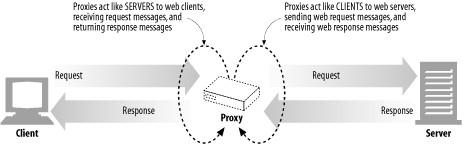
\includegraphics[width=310px]{img/proxy_1}
	\caption{\small Esquema del funcionamiento de un proxy, extra'ido de \cite{httpGuide}}
	\label{proxy_1}
\end{figure}

El esquema de la Figura \ref{proxy_1} muestra una conexi'on utilizando HTTP, las peticiones viajan directamente al proxy y de ah'i al servidor final. En el caso de HTTPS se hace de manera diferente. Primero el cliente env'ia una petici'on con el M'etodo CONNECT que incluye la direcci'on y el puerto del destino final. El proxy autentica la conexi'on, completa la negociaci'on con el destino y responde al cliente con un mensaje que contiene el c'odigo 200 que indica que la conexi'on fu'e establecida. Luego, el proxy se convierte en un t'unel que solo reenv'ia los paquetes del cliente hacia el servidor y viceversa (todo el tr'afico se encuentra encriptado). Esto puede ilustrarse en la Figura \ref{proxy_2}.
\label{mitm}
Los browsers actuales no soportan proxies HTTP Seguros, es decir, que se establezca una sesi'on SSL del cliente al proxy y otra del proxy al servidor final como puede verse en la Figura \ref{trustedProxy}. Este 'ultimo punto est'a en discusi'on, se propuso un borrador \citep{draftTrustedProxy} al respecto.

\begin{figure}[h]
  	\centering
	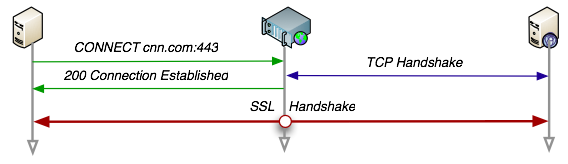
\includegraphics[width=\textwidth]{img/proxy_2}
	\caption{\small T'unel HTTPS sobre un Proxy, extra'ido de \cite{secureProxies}}
	\label{proxy_2}
\end{figure}

\begin{figure}[h]
  	\centering
	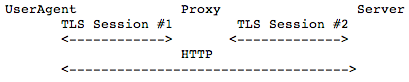
\includegraphics[width=\textwidth]{img/trustedProxy}
	\caption{\small T'unel HTTPS sobre un Proxy, extra'ido de \cite{draftTrustedProxy}}
	\label{trustedProxy}
\end{figure}

\section{Usos de un Proxy}

Hay diversas utilizaciones de los servidores proxy, entre ellas se destacan:

\begin{enumerate}
\item Proxy NAT\footnote{Network Address Translation.} / Enmascaramiento

El enmascaramiento IP o tambi'on llamado traducci'on de direciones de red, es el proceso por el cual las direcciones IP del origen/destino son reescritas, se sustituyen por otras. Es 'util cuando se dispone de una 'unica direcci'on p'ublica que se comparte entre varios usuarios. El proxy se encarga de enmascarar las direcciones privadas de los clientes, traduciendol'a a la direcci'on p'ublica, para realizar las peticiones al exterior. Cuando recibe la respuesta de los servidores exteriores, se encarga de derivarla al usuario que inici'o el pedido.

\item Filtro

El Proxy al recibir las peticiones de los clientes, puede permitir o denegar esas peticiones seg'un ciertas pol'iticas definidas. Por ejemplo, en una Instituci'on Educativa se podr'ia bloquear el acceso a ciertas redes sociales o sitios para adultos.

\item Cortafuegos\footnote{Firewall.}

Al ser un intermediario, y muchas veces como puerta de acceso hacia internet, se pueden utilizar para aumentar el nivel de seguridad restringiendo ciertos protocolos o filtrando cierto contenido inseguro por ejemplo.

\item Web Cach'e

Puede utilizarse para mantener copias locales de los recursos peticionados por los clientes, y al momento de recibir una petici'on por un recurso que se encuentra almacenado, se brinda esa copia al cliente. Al servir varios clientes esto incrementa la velocidad de respuesta. Es uno de los usos m'as importantes de un proxy, ya que reduce notablemente los tiempos de carga de los sitios cuando se produce un cach'e Hit. Esto se ver'a detalladamente en el Cap'itulo \ref{cache}.

\item Proxy Reverso / Surrogate Server

Puede actuar delante de un servidor web, atendiendo peticiones de los clientes como si fuera 'el Servidor mismo. Esto permite por ejemplo, generar una Red de Distribuci'on de Contenidos (CDN). Recibe una petici'on de un cliente, y, en vez de devolver el contenido directamente, inicia una comunicaci'on con otros servidores para localizar el recurso pedido, de manera m'as eficiente. Tambi'en protege a los servidores web, a'nadiendo una capa adicional de defensa. Puede distribuir la carga entre varios servidores web.

\item Content-Router

Pueden redirigir las peticiones a diferentes Servidores, basados en las condiciones del Tr'afico de Internet y el tipo de contenido.

\item Transcoder

Puede modificar el contenido de los recursos antes de hacer el env'io a los clientes. Por ejemplo, transformar im'agenes BMP a JPEG para reducir el tama'no, comprimir archivos de texto, e incluso hacer una traducci'on del contenido a otro lenguaje.

\item Anonimizador

Permite navegar de manera privada y an'onima removiendo ciertos datos de los mensajes HTTP (direcci'on IP, From header, cookies, etc).

\end{enumerate}

\section{Ventajas y Desventajas}

\subsection{Ventajas}

\begin{enumerate}
\item Control

Al ser intermediario, es el proxy el 'unico que va a realizar el trabajo de comunicaci'on hacia el exterior, es el que tiene la potestad de limitar y restringir los derechos de los clientes, ya que todo pasa a trav'es de 'el.
\clearpage
\item Optimizaci'on de los tiempos de carga

En el caso de los proxies que ofrecen servicio de cach'e, se optimizan los tiempos de carga de los sitios, al tener almacenada copias locales que puede brindar directamente al usuario sin tener que realizar la petici'on al servidor final.
\item Optimizaci'on del uso de recursos

El proxy es el 'unico que realiza el trabajo hacia afuera, es decir, que al utilizar una sola conexi'on, se maximiza el uso del ancho de banda.
\item Modificaci'on de la Informaci'on

Al tener acceso a los recursos que viajan a trav'es de 'el, tiene la posibilidad de modificarlos.
\item Filtrado

Recibir todas las peticiones del usuario, da la posibilidad de poder decidir que recursos o qu'e sitios son los que est'an habilitados para su recuperaci'on. Podr'ia manejarse una lista negra\footnote{Listado de sitios a los que NO se puede acceder.} o una lista blanca\footnote{Listado de sitios cuyo acceso est'a permitido.} por ejemplo.

\item Tr'afico controlado

Debido a que todo el tr'afico pasa a trav'es del proxy, se puede registrar un gran volumen de informaci'on que luego puede usarse para auditor'ia y seguridad.
\item Anonimato

Permite a los usuarios acceder a los servicios que brinda Internet, protegiendo la red interna. Al acceder al exterior identific'andose como el mismo, es dif'icil para el recurso diferenciar quien es el que est'a realizando la petici'on.
\end{enumerate}
\clearpage
\subsection{Desventajas}

\begin{enumerate}
\item M'ultiples funciones

Al estar a disposici'on de todas las peticiones de los usuarios, es posible que tenga que realizar algunas tareas no espec'ificas de su funci'on, por ejemplo los controles de acceso a sus servicios.
\item Carga de trabajo

Al ser el intermediario de todos los usuarios, el proxy tiene que realizar el trabajo de todos ellos. La carga de trabajo crece en la medida en que crezcan la cantidad de usuarios que consumen sus servicios.
\item Confianza del Usuario

Pueden aparecer usuarios que no se sientan c'omodos con que todo su tr'afico sea interceptado. Adem'as, todas las transacciones realizadas se guardan en archivos de logs\footnote{Registro oficial de eventos durante un rango de tiempo en particular.}, es decir que toda la actividad que el usuario realice a trav'es del proxy quedan registradas. En una conexi'on sin intermediarios, es imposible tener la informaci'on completa de las transacciones realizadas ya que se encuentra esparcida en servidores diseminados por todo el mundo.
\item Modificaci'on en el Software de los usuarios

La utilizaci'on de un proxy, requiere que las aplicaciones que interact'uan con Internet que los usuarios utilizan en la red interna, se configuren (Ver Secci'on \ref{proxyConf}) para que puedan tener acceso hacia el exterior a trav'es del proxy. 
\item Servicios no disponibles

Existen algunos aplicaciones que no funcionan con un proxy de por medio, por ejemplo el servicio de mensajer'ia Whatsapp\footnote{http://www.whatsapp.com/}.
\item Retardo

Que la comunicaci'on del cliente con el servidor final no sea directa, supone un retardo en las comunicaciones, que muchas veces se ve compensado si alg'un objeto se encuentra en la cach'e del proxy.
\end{enumerate}

\section{Configuraci'on}
\label{proxyConf}
Existen varias maneras de configurar un browser para navegar a trav'es de un proxy.
\begin{enumerate}
\item Manual: Se configura desde una opci'on espec'ifica del navegador.
\item Flags\footnote{Bandera}: Un proxy puede configurarse con un flag espec'ifico en el lanzamiento del proceso, esto permite indicar el proxy previo a la ejecuci'on del navegador. En el caso de Google Chrome / Chromium el flag utilizado es:
\begin{quote}
\textit{--proxy-server direccion:puerto}
\end{quote}
Este flag es el que se va a utilizar m'as adelante en la parte de experimentaci'on del proxy desarrollado. El listado de banderas completo se encuentra online\footnote{http://peter.sh/experiments/chromium-command-line-switches/}.
\item Archivos PAC\footnote{Proxy Auto-Configuration.}: Puede definirse un archivo de Auto-Configuraci'on de proxy, es un archivo Javascript en el que se pueden realizar acciones avanzadas como por ejemplo, identificar los protocolos y redireccionar al proxy indicado. Ejemplo de archivo PAC en el que se direcciona seg'un el protocolo (HTTP, HTTPS a un proxy diferente):
\begin{quote}
function FindProxyForURL(url, host) \{

\hspace{1cm}if (url.substring(0,5) == "http:") \{

        \hspace{2cm}return "PROXY proxy.normal.com:8080";
        
\hspace{1cm}\}else if (url.substring(0,6) =="https:") \{

	\hspace{2cm}return "PROXY proxy.seguro.com:8080";
	
\hspace{1cm}\} else \{

        \hspace{2cm}return "DIRECT";
        
    \}
\end{quote}
\end{enumerate}
\chapter{Cach'e Web}
\label{cache}
\section{Definici'on}

Un cach'e web es un intermediario entre un cliente (o varios) y un Servidor (o varios). Observa las peticiones que se van realizando y va almacenando los recursos solicitados, de manera que, si hay otra petici'on de la misma \textsc{url}, el intermediario puede brindar el recurso sin tener que solicitarlo al destino original \citep{cacheDef}.

El funcionamiento b'asico de un Cach'e es el siguiente. Cuando se recibe una petici'on del cliente, se busca el recurso en el almacenamiento local. En el caso de encontrarlo, se realiza la verificaci'on de que el recurso est'e ''fresco'', es decir, que la copia se encuentre actualizada. Luego, se env'ia como respuesta al cliente, la copia local. Cuando el recurso se devuelve desde la cach'e, se llama Cach'e HIT\footnote{Acierto}, y, en el caso de que el recurso no se encuentre, se llama Cach'e MISS\footnote{Desacierto}.
\vspace{5mm}

Posee ciertos beneficios al proveer un mecanismo eficiente para la distribuci'on de Informaci'on en la Web \citep[p. 20]{webCaching}.
\begin{enumerate}
\item Latencia

Un Cach'e Web cercano a los clientes, reduce la latencia para los aciertos de cach'e\footnote{Cuando un recurso solicitado por el cliente, efectivamente se encuentra almacenado en la cach'e.}. Los retrasos en la transmisi'on son menores por la cercan'ia entre los dos puntos de interacci'on. Adicionalmente, se reducen los retrasos por retransmisi'on y las esperas en los routers a causa de que hay menos enlaces intermedios involucrados.
\item Ancho de Banda

Cuando se utilizan las copias de los recursos almacenados en la cach'e, se ahorra ancho de banda, ya que no hay que hacer la petici'on del recurso al destino final.
\item Carga del Servidor

Reduce la carga de los servidores al disminuir la cantidad de peticiones que se realizan. Un servidor que esta con poca carga de trabajo es m'as r'apido que uno que est'a muy ocupado, es decir, atendiendo gran cantidad de peticiones de diferentes clientes.

\item Si un servidor remoto no est'a disponible temporalmente, una copia del objeto pedido se puede recuperar de la cach'e.
\end{enumerate}

\section{Tipos}

Hay diferentes tipos de Cach'es Web, entre ellos se encuentran los siguientes:

\begin{enumerate}
\item Cach'e de Navegador

Los navegadores tienen un cach'e incluido, la informaci'on se almacena de manera local en el dispositivo del usuario. Esta limitado a 1 solo usuario, y se obtiene un hit de cach'e, solamente cuando se visita nuevamente algun sitio que ya se haya visitado.
\item Proxy Cach'es

A diferencia de los de navegador, estos sirven a un n'umero grande de usuarios. Al crecer la cantidad de usuarios, tambi'en crece la tasa de aciertos de la cach'e, ya que los usuarios suelen acceder a los mismos sitios (sitios de gran popularidad) \citep{duska}.
\item Surrogates Servers

Son intermediarios que act'uan con la autoridad del servidor original para servir contenidos como si fueran el servidor mismo \citep{edgeArch}. Generalmente se encuentran cerca de los servidores originales, sirviendo el contenido de los mismos, generalmente desde una cach'e interna.

Se usan como Redes de Distribuci'on de Contenidos (CDN), para tener replicaciones de los recursos de un servidor en diferentes lugares. Los recursos peticionados por los clientes, son revueltos por el CDN m'as cercano fisicamente. Tambi'en se usan como aceleradores, simplemente almacenando en la cach'e las respuestas del servidor.
\end{enumerate}

\section{Politicas de Reemplazo / Algoritmos de Cach'e}

Para el buen funcionamiento de la cach'e, hay que definir de qu'e manera se van reemplazando los contenidos almacenados en la misma. Para esto se utiliza una Pol'itica de Reemplazo de objetos, orientado a ciertas caracter'isticas de los objetos, tales como el tama'no, cantidad de peticiones de dicho objeto, tiempo almacenado en la cach'e, etc.
Hay diversos algoritmos que se detallan a continuaci'on.
%\citep{reempCache}
\begin{enumerate}
\item Primero en Entrar Primero en Salir (FIFO\footnote{First In First Out})

Este m'etodo es el m'as sencillo, se trata de una cola en la que el primer elemento en entrar es el primer elemento en salir, es decir, aquel que m'as tiempo haya estado en la cach'e es el que m'as probabilidades tiene de salir.
\item Aleatorio

Realiza el reemplazo buscando aleatoriamente un objeto almacenado en la cach'e.
\item Menos Usado Recientemente (LRU\footnote{Last Recently Used})

Este m'etodo, busca reemplazar al objeto que m'as tiempo haya estado en la cach'e sin ser peticionado, es decir, aquel objeto que menos peticiones haya tenido en un lapso de tiempo amplio, es el que tiene m'as posibilidades de ser reemplazado.
\item Menor Menos Usado Recientemente (LRU-MIN)

Es una optimizaci'on del algoritmo LRU, en el cual se busca reemplazar los objetos de mayor tama'no de la cach'e. quedando as'i objetos de menor tama'no almacenados.
\item Menos Frecuentemente Usado (LFU\footnote{Least Frequently Used})

Se eval'ua la frecuencia con la que un elemento es solicitado, el que es menos solicitado es el que tiene m'as posibilidades de ser reemplazado.
\end{enumerate}

\section{Control de Cach'e}
\label{controlCache}

Cuando el cliente realiza una petici'on, y esta coincide con un elemento que tenemos almacenado en la Cach'e se debe evaluar si es viable enviar la copia local, o hacer la petici'on nuevamente, a esto se le llama Revalidaci'on. Para esto se realizan ciertos controles (extra'idos de \citep{cacheDef}) en base a los Headers de HTTP (vistos en \ref{headers}).

\begin{enumerate}
\item El Header \textsl{Expires}, nos indica cuanto tiempo va a estar ''fresco''\footnote{No va a tener cambios.} el recurso. Si en el momento de la petici'on, todav'ia no expir'o el recurso, puedo servirlo de la copia local. Tiene algunas limitaciones, como por ejemplo que el valor permitido es una fecha en GMT, lo que lleva a que los relojes del Servidor y del cach'e est'en sincronizados, de otra manera no tiene sentido una comparaci'on de fechas. Otro problema que se encuentra es que si se env'ia este header, pero no est'a actualizado, siempre va a enviar una fecha anterior a la actual lo que llevar'ia a generar siempre la petici'on del recurso.
\item Se puede utilizar el Header \textsl{Cache-control}\footnote{Implementado a partir de la versi'on 1.1 de HTTP} que brinda informaci'on variada. El formato es: \textbf{Cache-control: especificaci'on1, especificaci'on2, especificaci'onN}.
	\begin{enumerate}
	\item \textsl{max-age} - Especifica en tiempo en el que el recurso puede ser considerado ''fresco'' en segundos. Es el similar a \textsl{Expires} pero con un valor espec'ifico a diferencia de una marca de tiempo.
	\item \textsl{s-maxage} - Similar al anterior pero para los cach'es compartidos\footnote{Por ejemplo un Proxy.}.
	\item \textsl{public} - Indica que las peticiones que requieren autenticaci'on pueden almacenarse en la cach'e.
	\item \textsl{private} - Permite que el recurso puede almacenarse en aquellos cach'es que son solo para 1 solo usuario\footnote{Por ejemplo la cach'e de un Browser.} y no en una cach'e compartida.
	\item \textsl{no-cache} - Fuerza a que el recurso tenga que revalidarse antes de devolver la copia local de la cach'e al cliente.
	\item \textsl{no-store} - Indica que el recurso no debe quedar almacenado en la cach'e bajo ninguna circunstancia.
	\item \textsl{must-revalidate} - Si el recurso luego de validarlo en la cach'e no esta ''fresco'', debe revalidarse.
	\item \textsl{proxy-revalidate} - Igual que \textsl{must-revalidate} pero aplicado a Proxies.
	\end{enumerate}
\end{enumerate}

Cuando ambos Headers, \textsl{Expires} y \textsl{Cache-control} est'an presentes en la respuesta, \textsl{Cache-control} es el que toma mayor importancia.

Para realizar la Revalidaci'on se utilizan ciertos Headers en la petici'on. Los Servidores utilizan 2 Headers para realizar las validaciones, uno es \textsl{Last-Modified}, que indica cu'ando fu'e modificado por 'ultima vez el recurso. Cuando 'este est'a presente, el cliente puede realizar una petici'on con el Header \textsl{If-Modified-Since}:fecha, para que el servidor devuelva el recurso unicamente si se cumple con esta condici'on, de no ser as'i, devuelve un mensaje con el c'odigo \texttt{304 Not Modified}, que indica que el recurso no fue modificado y se puede servir la copia local.
Por otro lado, se utiliza un identificador llamado \textsl{ETag} que se genera cada vez que el recurso se modifica. Es una cadena de texto que identifica una versi'on espec'ifica del recurso. En este caso, el cliente puede utilizar el Header \textsl{If-None-Match}:ETag\_local, que el servidor responde con el recurso en el caso de que el identificador enviado por el cliente no coincida con el del objeto peticionado.
\chapter{SpdyProxyPython}
\label{spdyproxypython}

\section{Introducci'on}

Ya conocido el crecimiento de Internet visto en el Cap'itulo \ref{desarrolloWeb}, las deficiencias de los protocolos visto en el Cap'itulo \ref{protocolos}, y la problem'atica de los tiempos de carga y sus posibles optimizaciones \ref{problematica}.
%CAPITULOS QUE FALTAN
\chapter{Desarrollo de spdyProxyPython}
\section{Como funciona}
\section{Features}
\section{pseudocodigo del arbol implementado}
\section{modulos adicionales}
cliente spdy, methodGuesser, rttMeasure, decisionTree
\chapter{Pruebas del Proxy}
\section{modulos adicionales}
alexatop, tester y parser
\section{como se va a probar}
\section{resultados}
\chapter{conclusiones}
%\include{capitulo2}
%\include{capitulo3}
%\include{conclu}

%ap'endices
%\appendix
\glossarystyle{altlistgroup}
\glsaddall
\printglossary[title=Glosario]

%bibliografia
\nocite{*}
\bibliography{biblio/biblio}

\end{document}
